\cotefile{79}
\scanpage{283}

\[
\begin{aligned}
(s,t)\in A_0&\Longleftrightarrow(s,\lambda t)\in A_\lambda\\
\mathrm{Et}_{A_0}(t)&=\mathrm{Et}_{A_\lambda}(\lambda t)
\end{aligned}
\]

\figure{\begin{tikzpicture}[x=.88cm,y=.78cm]
\draw (0,0)--(1,0) (1.6,0)--(3.15,0);
\draw (2.5,1.9) .. controls (3.65,.8) and (3.45,-1.35) .. (2.43,-2.0);
\draw[->] (2.85,1.10)..controls (3.44,0) and (3.2,-1.53)..(2.43,-2.0);
\draw (3.53,.13)--(6.69,1.95) (3.68,-.49)..controls (4.59,-1.10) and (5.81,-1.80)..(6.69,-1.93);
\draw (7.42,2.56)..controls (5.82,1.63) and (5.55,-2.04)..(7.83,-2.62);
\draw[->] (6.14,.15)..controls (6.19,1.11) and (6.43,1.65)..(6.70,1.94);
\draw (6.22,.05)--(8.18,0);
\foreach \x/\y in {0/0,2.5/1.9,2.43/-2,3.15/0,3.44/.14,6.22/.05,6.69/1.95,6.69/-1.93,8.18/0}{\fill (\x,\y) circle (1.15pt);}
\node[below right] at (-.1,0) {$\sigma t$}; \node at (1.35,0) {$s$};
\node[above] at (2.60,1.92) {$t'$}; \node[below right] at (2.40,-1.9) {$t''$};
\node at (3.49,-.05) {$t$}; \node[left] at (6.22,.05) {$\lambda t$};
\node[above left] at (6.78,2.02) {$t'$}; \node[below left] at (6.81,-1.89) {$t''$};
\node[right] at (8.18,0) {$\underset{\substack{\shortparallel\\s'}}{\lambda^{-1}s}$};
\draw[->] (4.00,3.10)--node[above] {$\lambda$} node[below] {$u_\lambda$} (5.04,3.10);
\draw[<-] (3.84,-2.54)--node[above] {$\lambda^{-1}$} node[below] {$u_{\lambda^{-1}}$} (5.07,-2.54);
\draw[->] (9.12,-.02)--(11.16,-.02); \draw[->] (10.10,-.18)..controls (10.25,.06) and (10.23,.30)..(10.15,.49);
\node at (.25,1.56) {$\checkmark$};
\end{tikzpicture}}

\[t'=\lambda t\dotplus\unsure{\nu|v}\ \big/\ t''=\lambda t-\nu\]

% margin note written sideways
\margin{$R_0\subset S\times S^*$}

\[\sigma(\lambda t)=\lambda\sigma(t)\quad\text{lié à }t\]

\figure{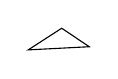
\begin{tikzpicture}[scale=.5]\draw (0,0)--(.85,.55)--(1.55,.08)--cycle;\end{tikzpicture}}

\[(s,t)\in A_0\Longleftrightarrow(s,\lambda t)\in A_\lambda\]

\[
\begin{aligned}
&\forall a,\ \unsure{\exists!|\exists}f\ \text{triangle, tel que}\quad a\in f\\
&\deleted{N/6}\ \operatorname{card} A=N/2\\
&\operatorname{card} F=(N/2)!
\end{aligned}
\]

$(a,f)$ en nb $\nu\,(N/2)$

donc il y a $\nu(N/2)/3$ faces

Si $\nu=1$, ça fait $N/6$ faces

\uline{le stabilisateur d'une face serait d'ordre $6$}

\figure{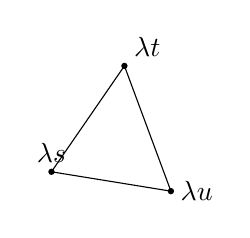
\begin{tikzpicture}[scale=.82]
\draw (0,0)--(1.13,1.64)--(1.85,-.30)--cycle;
\foreach \x/\y in {0/0,1.13/1.64,1.85/-.30}{\fill (\x,\y) circle (1.4pt);}
\node[above] at (0,0) {$\lambda s$};\node[above right] at (1.13,1.64) {$\lambda t$};
\node[right] at (1.85,-.30) {$\lambda u$};
\end{tikzpicture}}

\[\boxed{\lambda t\underset{\substack{s'\\\shortparallel\\\lambda^{-1}s}}{\overset{\cdot}{\pm}}\nu\ \text{est incident à }t}\]

\[
\begin{aligned}
\lambda(t\underset{s}{\dotplus}\zeta)\pm\nu&\ \text{est incident : }t+\zeta\\
\lambda t\underset{s'}{\dotplus}\underbrace{\lambda^2\zeta\pm\nu}&\ \rule{2cm}{.3pt}\ t+\zeta\\
\zeta'&=\lambda^2\zeta\pm\nu\\
\zeta&=\lambda^{-2}\zeta'\pm\lambda^{-2}\cdot\nu
\end{aligned}
\]

\[\lambda^{-2}\nu=\nu^{-1}\]

% margin note written sideways
\margin{\unsure{irréelle|ivréelle} \deleted{dans} au beau milieu de ce délire mathématico-philoso}

% archive sheet number: 282
\scanpage{284}

\figure{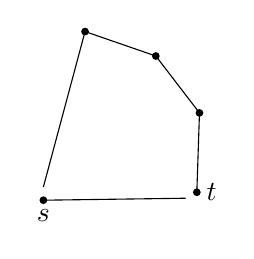
\begin{tikzpicture}[x=.84cm,y=.84cm]
\draw (0,.20)--(.63,2.55)--(1.7,2.18)--(2.36,1.32)--(2.32,.12); \draw (0,0)--(2.15,.03);
\foreach \x/\y in {0/0,.63/2.55,1.7/2.18,2.36/1.32,2.32/.12}{\fill (\x,\y) circle (1.4pt);}
\node[below] at (0,0) {$s$}; \node[right] at (2.32,.12) {$t$};
\end{tikzpicture}}

\[
\begin{aligned}
&\forall s\in S,\quad \exists s'\in S\\
&\text{tel que }\mathrm{Et}_{A_0}(s)=\mathrm{Et}_{A}(s')
\end{aligned}
\]

\figure{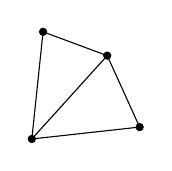
\begin{tikzpicture}[x=.84cm,y=.84cm]
\draw (0,0)--(.17,1.62)--(1.14,1.26)--(1.63,.18)--cycle (0,0)--(1.14,1.26);
\foreach \x/\y in {0/0,.17/1.62,1.14/1.26,1.63/.18}{\fill (\x,\y) circle (1.5pt);}
\end{tikzpicture}}

\figure{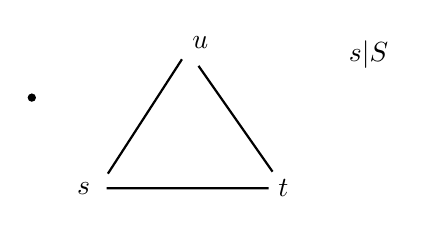
\begin{tikzpicture}[x=.84cm,y=.84cm]
\draw[thick] (.12,.22)--(1.24,1.95) (1.49,1.85)--(2.61,.25) (.10,0)--(2.55,0);
\node[left] at (0,0) {$s$};\node[right] at (2.55,0) {$t$};\node[above right] at (1.25,1.96) {$u$};
\fill (-1.03,1.37) circle (1.5pt); \node at (4.06,2.02) {$\unsure{s|S}$};
\end{tikzpicture}}

\figure{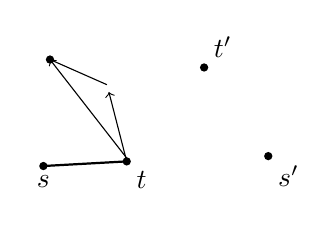
\begin{tikzpicture}[x=.84cm,y=.84cm]
\draw[thick] (0,0)--(1.26,.07);
\draw[->] (1.26,.07)--(.99,1.12); \draw[->] (1.26,.12)--(.10,1.61); \draw (.10,1.61)--(.96,1.23);
\foreach \x/\y in {0/0,1.26/.07,.10/1.61,2.43/1.49,3.40/.15}{\fill (\x,\y) circle (1.5pt);}
\node[below] at (0,0) {$s$};\node[below right] at (1.26,.07) {$t$};
\node[above right] at (2.43,1.49) {$t'$};\node[below right] at (3.40,.15) {$s'$};
\end{tikzpicture}}

\figure{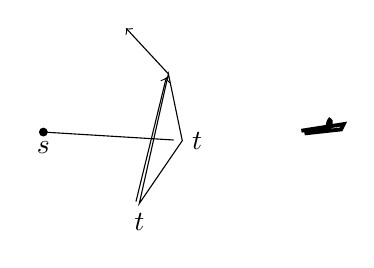
\begin{tikzpicture}[x=.84cm,y=.84cm]
\draw (0,0)--(1.97,-.12) (1.45,-1.08)--(2.10,-.13)--(1.89,.88)--cycle;
\draw[->] (1.40,-1.05)--(1.86,.83); \draw[->] (1.89,.88)--(1.25,1.57);
\fill (0,0) circle (1.6pt); \node[below] at (0,0) {$s$};\node[right] at (2.1,-.13) {$t$};\node[below] at (1.45,-1.08) {$t$};
\draw[line width=1.4pt] (3.9,.02)--(4.54,.12)--(4.50,.04)--(3.95,-.02)--(4.33,.08) .. controls (4.38,.24) and (4.28,.22) .. (4.30,.00);
\end{tikzpicture}}

\figure{\begin{tikzpicture}[x=.84cm,y=.84cm]
\draw[thick] (.22,0)--(2.41,.06) (2.94,.07)--(5.31,.16) (5.92,.18)--(7.21,.19);
\draw (5.61,.52)--(5.86,1.77); \fill (5.23,1.83) circle (1pt); \node[above right] at (5.23,1.83) {$t'$};
\node at (0,0) {$s$};\node at (2.65,.05) {$t$};\fill (5.57,.18) circle (1pt);
\node[below right] at (5.38,.18) {$\deleted{\lambda t}\,\lambda t$};\fill (7.48,.2) circle (1.4pt);
\node[right] at (7.48,.2) {$s'=\lambda^{-1}s$};
\end{tikzpicture}}

\figure{\begin{tikzpicture}[x=.84cm,y=.84cm]
\draw (.20,0)--(2.78,.20) (3.53,.29)--(6.6,1.82);
\node at (0,.06) {$s$}; \node at (3.05,.21) {$t$}; \fill (6.62,1.91) circle (1.2pt);
\node[above left] at (6.62,1.91) {$t'$};\fill (6.20,.43) circle (1pt); \fill (9.22,.63) circle (1pt);\node[right] at (9.22,.63) {$s'$};
\end{tikzpicture}}

% archive sheet number: 283
\scanpage{285}

\[
\begin{aligned}
gaU&=g'aU\quad\text{si }gU=g'U\ \text{i.e.}\quad g'^{-1}g\in U\\
a^{-1}(g'^{-1}g)a\deleted{U}&\in U\quad\text{si }g'^{-1}g\in U\\
&a^{-1}Ua
\end{aligned}
\]

\figure{\begin{tikzpicture}[x=0.008cm,y=-0.008cm]
\draw (0,0)--(90,47)--(86,148);
\end{tikzpicture}}

\[
x\qquad\lambda x
\]

\figure{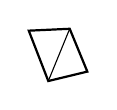
\begin{tikzpicture}[x=0.008cm,y=-0.008cm]
\draw[thick] (0,0)--(65,-3)--(93,65)--(31,80)--cycle;
\draw (31,80)--(65,-3);
\end{tikzpicture}}

\figure{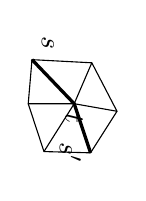
\begin{tikzpicture}[x=0.008cm,y=-0.008cm]
\draw (0,0)--(95,5)--(135,82)--(93,148)--(19,146)--(-6,70)--cycle;
\draw[very thick] (0,0)--(67,70)--(93,148);
\draw (95,5)--(67,70)--(19,146);
\draw (-6,70)--(67,70)--(135,82);
\node[above left,rotate=-90] at (0,0) {$s$};
\node[right,rotate=-90] at (67,70) {$t$};
\node[below,rotate=-90] at (93,148) {$s'$};
\end{tikzpicture}}

\[
\begin{aligned}
\underset{\substack{\shortparallel\\ B}}{G_{\unsure{x_0|s_0}}}
=G_s=\underset{\substack{\shortparallel\\\mathrm{int}(g)\,B}}{G_{g\cdot s_0}}
\end{aligned}
\]

\figure{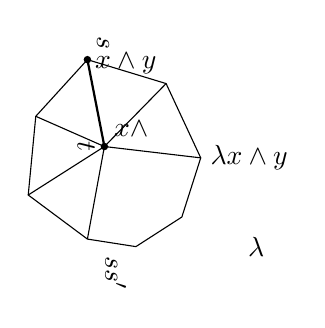
\begin{tikzpicture}[x=0.008cm,y=-0.008cm]
\draw (100,0)--(225,38)--(280,156)--(250,250)--(177,297)--(100,285)--(6,215)--(18,90)--cycle;
\draw[thick] (100,0)--(127,138);
\draw (225,38)--(127,138)--(280,156);
\draw (18,90)--(127,138)--(100,285);
\draw (6,215)--(127,138);
\fill (100,0) circle[radius=1.35pt];
\fill (127,138) circle[radius=1.35pt];
\node[above left,rotate=-90] at (100,0) {$s$};
\node[below,rotate=-90] at (127,138) {$t$};
\node[below right,rotate=-90] at (177,297) {$\deleted{\unsure{s}}s'$};
\node[above left] at (225,38) {$x\wedge y$};
\node[above right] at (127,138) {$\deleted{x\wedge}$};
\node[right] at (280,156) {$\deleted{\lambda x\wedge y}$};
\node[right=13mm] at (177,297) {$\lambda$};
\end{tikzpicture}}

\[
\begin{aligned}
x\wedge y=e&\Rightarrow x\wedge\overbrace{\lambda y}^{y'}=\lambda e\\
&\lambda^{-1}x\wedge y'=e
\end{aligned}
\]

\figure{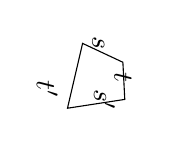
\begin{tikzpicture}[x=0.008cm,y=-0.008cm]
\draw (24,0)--(88,30)--(91,89)--(0,103)--cycle;
\node[above,rotate=-90] at (24,0) {$s$};
\node[right,rotate=-90] at (88,30) {$t$};
\node[below,rotate=-90] at (91,89) {$s'$};
\node[below left,rotate=-90] at (0,103) {$t'$};
\end{tikzpicture}}

\figure{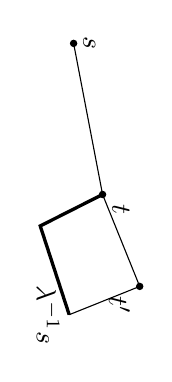
\begin{tikzpicture}[x=0.008cm,y=-0.008cm]
\draw (53,-240)--(99,0)--(158,146)--(46,191);
\draw[very thick] (46,191)--(0,50)--(99,0);
\fill (53,-240) circle[radius=1.35pt];
\fill (99,0) circle[radius=1.35pt];
\fill (158,146) circle[radius=1.35pt];
\node[above,rotate=-90] at (53,-240) {$s$};
\node[above right,rotate=-90] at (99,0) {$t$};
\node[below right,rotate=-90] at (158,146) {$t'$};
\node[below,rotate=-90] at (46,191) {$\lambda^{-1}s$};
\end{tikzpicture}}

\figure{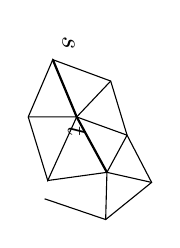
\begin{tikzpicture}[x=0.008cm,y=-0.008cm]
\draw (32,0)--(124,34)--(150,120)--(189,195)--(116,254)--(19,221);
\draw (-7,91)--(32,0)--(70,91)--(124,34);
\draw (-7,91)--(70,91)--(150,120)--(118,179)--(189,195);
\draw[thick] (32,0)--(70,91)--(118,179);
\draw (-7,91)--(24,192)--(70,91);
\draw (24,192)--(118,179)--(116,254);
\node[above left,rotate=-90] at (32,0) {$s$};
\node[right,rotate=-90] at (70,91) {$t$};
\end{tikzpicture}}

\figure{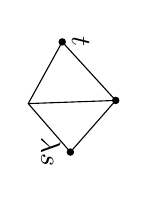
\begin{tikzpicture}[x=0.008cm,y=-0.008cm]
\draw (54,0)--(139,93)--(67,175)--(0,98)--cycle;
\draw (0,98)--(139,93);
\fill (54,0) circle[radius=1.35pt];
\fill (139,93) circle[radius=1.35pt];
\fill (67,175) circle[radius=1.35pt];
\node[above,rotate=-90] at (54,0) {$t$};
\node[below,rotate=-90] at (67,175) {$\lambda s$};
\end{tikzpicture}}

\[
\begin{aligned}
\underset{\shortparallel}{\mathrm{Et}_{A_0}(s)}&\xrightarrow{\lambda}\mathrm{Et}_{A_0}(\lambda^{-1}s)\\
\{y\mid x\wedge y=e\}&\qquad\{y'\mid\lambda^{-1}x\wedge y'=e\quad\text{i.e. }x\wedge y'=\lambda e\}\\
&y\longmapsto y'=\lambda y
\end{aligned}
\]

\figure{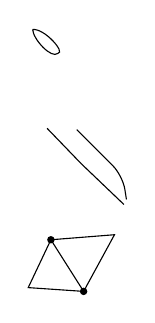
\begin{tikzpicture}[x=0.008cm,y=-0.008cm]
\draw (0,0) .. controls (19,-2) and (53,37) .. (40,38) .. controls (30,47) and (1,16) .. (0,0);
\draw[rounded corners=5pt] (70,159)--(143,232)--(149,270);
\draw (23,157)--(77,213);
\draw (77,213)--(145,278);
\draw (29,334)--(130,326)--(81,416)--(-7,410)--cycle;
\draw (29,334)--(81,416);
\fill (29,334) circle[radius=1.35pt];
\fill (81,416) circle[radius=1.35pt];
\end{tikzpicture}}

\[
{\rho}^{-1}(u)\,\rho^{-1}(a^{-1})\,a^{-1}
\]

\[
\begin{aligned}
y&\longmapsto y+x &\deleted{\lambda\unsure{v|x}}\quad y_1&=y+x\\
y'&\longmapsto y'+\lambda^{-1}x &\deleted{y'_1=y'+\lambda}&\\
&&\underset{y'_1}{\underline{\lambda y_1}}&=\underset{y'}{\underline{\lambda y}}+\lambda x=\\
&&y'_1&=y'+\lambda^2(\lambda^{-1}x)
\end{aligned}
\]

\figure{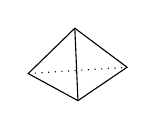
\begin{tikzpicture}[x=0.008cm,y=-0.008cm]
\draw (0,72)--(74,0)--(157,62)--(79,115)--cycle;
\draw (74,0)--(79,115);
\draw[dotted] (0,72)--(157,62);
\end{tikzpicture}}

\[
\begin{aligned}
\unsure{\rho_\infty|\beta_\infty|\rho_0}U&=h_\infty U & \tau_0\ \tau_1\\
h_\infty^{-1}\tau_0&\in U &\tau_1\\
\tau_0\underset{h_\infty}{\underbrace{\tau_1\tau_0}}&\in\underset{\substack{\shortparallel\\\langle\tau_1,\tau_{\unsure{2|\infty}}\rangle}}{U} &\mathrm{Et}(s)&=\\
\tau_0\tau_1\tau_0&\quad\therefore
\end{aligned}
\]

\[
\begin{aligned}
(s,t)&\qquad s,t &\{s,t\}\in A_0&\Longleftrightarrow\{s,\lambda t\}\in A_\lambda\\
\mathrm{Et}_{A_0}(t)&=\mathrm{Et}_{A_\lambda}(\lambda t) &&\mathrm{Et}(s)\cap\mathrm{Et}(\lambda t)
\end{aligned}
\]

\[
\begin{aligned}
\{s,\deleted{\unsure{\lambda}}t\}&\in A_0 &(s,t)&\in A_\lambda\\
\{s,\lambda^{-1}u\}&\in A_0 &(s,u\}&\in A_\lambda\\
\{t,\lambda^{-1}u\}&\in A_0 &(t,u)&\in A_\lambda
\end{aligned}
\]

\figure{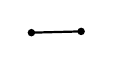
\begin{tikzpicture}[x=0.008cm,y=-0.008cm]
\draw[thick] (0,0)--(79,-2);
\fill (0,0) circle[radius=1.35pt];
\fill (79,-2) circle[radius=1.35pt];
\end{tikzpicture}}

% archive sheet number: 284
\scanpage{286}

\[
\begin{aligned}
a{\rho}^{-1}a\rho&\in\widetilde U\rho^{-1}(\tilde u)\\
&\deleted{a\rho^{-1}(a)\in}\\
av^{-1}\rho^{-1}a\rho v&\in\widetilde U\rho^{-1}(\widetilde U)\\
\deleted{av^{-1}a^{-1}}a\rho^{-1}a\rho v&\in\widetilde U(\rho v)^{-1}(\widetilde U)\\
&\widetilde{\deleted{a}}\,\overline{v^{-1}\rho^{-1}\widetilde U}\rho v
\end{aligned}
\]

\[
\begin{aligned}
\rho(a)a&\in\rho(\widetilde U)\widetilde U\\
\rho(ua)a&\in U\\
\deleted{\rho(a)a^{-1}(a)}&\quad\rho(ua)(av)\\
\rho(a)av&\in U_1 U_0\\
&\unsure{\rho(a)|g(a)}
\end{aligned}
\]

% margin note written sideways
\margin{$\mathrm{Et}_{A_0}(s)\cap\mathrm{Et}_{A_0}(\lambda^{-1}t)\ne\varnothing$}

\figure{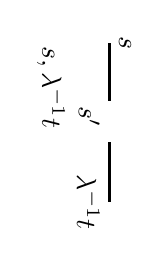
\begin{tikzpicture}[x=0.008cm,y=-0.008cm]
\draw[thick] (0,0)--(0,92);
\draw[thick] (0,157)--(0,252);
\node[above,rotate=-90] at (0,0) {$s$};
\node[below=2mm,rotate=-90] at (0,92) {$s'$};
\node[below,rotate=-90] at (0,252) {$\lambda^{-1}t$};
\node[left,rotate=-90] at (-93,150) {$s,\lambda^{-1}t$};
\end{tikzpicture}}

\[
\rho\qquad\overset{\frown}{U_0\quad U_1}\quad U_\infty
\]

\[
\begin{pmatrix}\lambda&\mu\\0&\lambda^{-1}\end{pmatrix}
\]

\figure{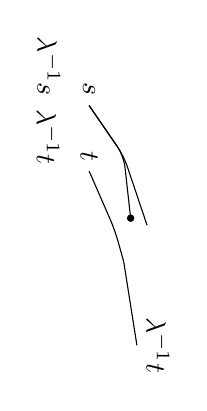
\begin{tikzpicture}[x=0.008cm,y=-0.008cm]
\draw[rounded corners] (0,0)--(55,80)--(66,179);
\draw[rounded corners] (0,0)--(55,80)--(92,190);
\draw[rounded corners] (0,104)--(41,198)--(55,248);
\draw (55,248)--(76,381);
\fill (66,179) circle[radius=1.35pt];
\node[left,rotate=-90] at (0,0) {$s$};
\node[left,rotate=-90] at (0,104) {$t$};
\node[left,rotate=-90] at (-64,0) {$\lambda^{-1}s$};
\node[left,rotate=-90] at (-65,110) {$\lambda^{-1}t$};
\node[above,rotate=-90] at (76,381) {$\lambda^{-1}t$};
\end{tikzpicture}}

\[
\begin{aligned}
\varepsilon_0=\sigma_\infty^{-1}\rho\qquad
\sigma_\infty(\varepsilon_0)&=\rho\,\sigma_\infty\\
\unsure{\rho_\infty|\rho}(\varepsilon_0)&=\rho\,\sigma_\infty^{-1}
\end{aligned}\ \bigg|\ \text{\unsure{définis|diffèrent} \unsure{par un|pour|par $\omega$}}
\]

\[
\begin{aligned}
\rho:\quad e_1&\longmapsto-e_2\\
\deleted{\unsure{e_1|e_\tau}}\!:\quad e_2&\longmapsto e_1+e_2\\
&\omega
\end{aligned}
\]

\figure{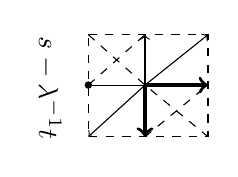
\begin{tikzpicture}[x=0.008cm,y=-0.008cm]
\draw[dashed] (0,0)--(90,0)--(190,0)--(190,80)--(190,162)--(90,162)--(0,162)--(0,80)--(0,0);
\draw[dashed] (0,0)--(90,80)--(190,162);
\draw[dashed] (0,80)--(90,0);
\draw[dashed] (90,162)--(190,80);
\draw[->] (90,80)--(90,0);
\draw[->] (90,80)--(190,0);
\draw[very thick,->] (90,80)--(190,80);
\draw[very thick,->] (90,80)--(90,162);
\draw[->] (90,80)--(0,162);
\draw (0,80)--(90,80);
\fill (0,80) circle[radius=1.35pt];
\node[rotate=-90] at (-62,85) {$s-\lambda^{-1}t$};
\end{tikzpicture}}

\[
\lambda^{-1}s=s\qquad\deleted{\unsure{s=s}}\qquad\deleted{\lambda^{-1}s=t}
\]

\figure{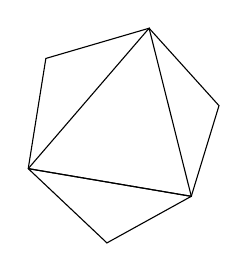
\begin{tikzpicture}[x=0.008cm,y=-0.008cm]
\draw (28,48)--(192,0)--(303,123)--(259,267)--(125,341)--(0,223)--cycle;
\draw (0,223)--(192,0)--(259,267)--(0,223);
\draw[thin] (0,223)--(259,267);
\end{tikzpicture}}

\[
\begin{pmatrix}1&0\\\mu&1\end{pmatrix}\begin{pmatrix}1&\mu'\\0&1\end{pmatrix}=\begin{pmatrix}1&\mu'\\\mu&1+\mu\mu'\end{pmatrix}
\]

\figure{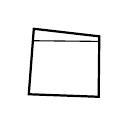
\begin{tikzpicture}[x=0.008cm,y=-0.008cm]
\draw[thick] (0,0)--(104,12)--(103,108)--(-8,104)--cycle;
\draw (-1,19)--(102,20);
\end{tikzpicture}}

% margin note written sideways
\margin{$E_0\quad E_0$}

\[
\rho=\begin{pmatrix}0&1\\-1&1\end{pmatrix}
\]

\[
\begin{aligned}
\underbrace{\begin{pmatrix}0&1\\-1&1\end{pmatrix}\begin{pmatrix}\lambda&0\\0&\lambda'\end{pmatrix}}\,
\underbrace{\begin{pmatrix}1&-1\\1&0\end{pmatrix}\begin{pmatrix}\lambda&0\\0&\lambda'\end{pmatrix}}
&=\begin{pmatrix}\lambda\lambda'&0\\\lambda\lambda'-\lambda^2&\lambda\lambda'\end{pmatrix}\\
\begin{pmatrix}0&\lambda'\\-\lambda&\lambda'\end{pmatrix}\begin{pmatrix}\lambda&-\lambda'\\\lambda&0\end{pmatrix}&=\begin{pmatrix}1&0\\1-\lambda^2&1\end{pmatrix}
\end{aligned}
\]

\[
\begin{aligned}\deleted{\mu=}\qquad\mu'&=0\\ \mu&=1-\lambda^{\unsure{2|\sim}}\end{aligned}
\]

\figure{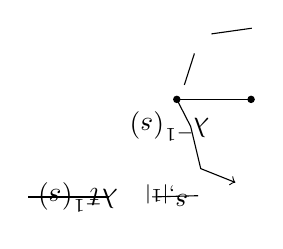
\begin{tikzpicture}[x=0.008cm,y=-0.008cm]
\draw (0,0)--(128,0);
\draw (197,0)--(270,-2);
\draw[->] (236,-155)--(258,-112)--(274,-45)--(329,-23);
\draw (236,-155)--(354,-155);
\draw (248,-178)--(264,-228);
\draw (291,-259)--(355,-268);
\fill (236,-155) circle[radius=1.35pt];
\fill (354,-155) circle[radius=1.35pt];
\node[left,rotate=180] at (0,0) {$\lambda^{-1}(s)$};
\node[right,rotate=180] at (128,0) {$t$};
\node[right,rotate=180] at (270,-2) {$s_{\unsure{,|1|{}}}$};
\node[left=9mm,rotate=180] at (258,-112) {$\lambda^{-1}(s)$};
\end{tikzpicture}}

% archive sheet number: 285
\scanpage{287}

\[
\begin{aligned}\mu(\lambda)&\in(\mathbb Z/n\mathbb Z)^*\\ \unsure{\nu|v}(\lambda)&\in(\mathbb Z/n\mathbb Z)/\pm1\qquad\nu\end{aligned}
\]

\diagram{\begin{tikzcd}[ampersand replacement=\&]
S\arrow[r,"\lambda^{-1}","\sim"']\arrow[d,"\mathrm{Et}_0"',"2"] \& S\arrow[d,"2"',"\mathrm{Et}_0"]\\
\deleted{\unsure{P}}\unsure{\mathcal E|\mathscr E}\arrow[r,"\sim","\lambda_{\mathcal E}"'] \& \deleted{\unsure{P}}\mathcal E\deleted{\unsure{ns}}
\end{tikzcd}}

\diagram{\begin{tikzcd}[ampersand replacement=\&]
S\arrow[r,"\overset{\mathrm{Et}_0}{\sim}"]\arrow[dr,"\mathrm{Et}_{\lambda}"'] \& \mathcal E\arrow[d,"?\,\lambda_{\mathcal E}"]\\
\&\mathcal E
\end{tikzcd}}

\figure{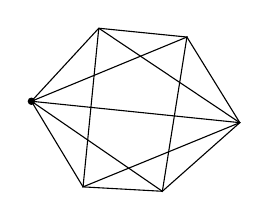
\begin{tikzpicture}[x=0.008cm,y=-0.008cm]
\draw (0,116)--(107,0)--(247,14)--(331,150)--(208,259)--(82,252)--cycle;
\draw (0,116)--(247,14)--(208,259)--(0,116);
\draw (107,0)--(82,252)--(331,150)--(107,0);
\draw[thin] (0,116)--(331,150);
\fill (0,116) circle[radius=1.35pt];
\end{tikzpicture}}

\[
E\qquad\deleted{R_E}\qquad\omega_E^\nu
\]

\[
\begin{aligned}\lambda\,\mathrm{Et}_0(s)&=\mathrm{Et}_0(\lambda^{-1}s)\\
\lambda\,\mathrm{Et}_0(s)&=\mathrm{Et}_\lambda(s)\qquad T_\lambda
\end{aligned}
\]

\[
(s,t)\ \overset{A_0}{\text{adj}}\ \Longrightarrow\ \lambda t\ \text{est }A_\lambda\text{-adj. à }\lambda t\underset{s,A_0}{\dotplus}\nu\ \overset{?}{\Longrightarrow}
\]

\[
\begin{aligned}\unsure{\lambda|\nu|\deleted{\nu}}\\
\deleted{(s,t)}\qquad\nu\ &\text{dépend de }\underline{A_0}\text{ et de }\lambda
\end{aligned}
\]

\figure{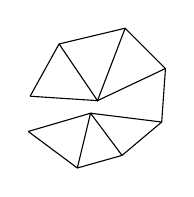
\begin{tikzpicture}[x=0.008cm,y=-0.008cm]
\draw (0,108)--(46,25)--(151,0)--(215,64)--(209,149)--(146,202)--(75,222)--(-3,164);
\draw (46,25)--(107,115)--(151,0);
\draw (215,64)--(107,115)--(0,108);
\draw (-3,164)--(96,135)--(75,222);
\draw (96,135)--(146,202);
\draw (96,135)--(209,149);
\end{tikzpicture}}

\[
\unsure{1|\vert}\quad \deleted{\unsure{S}}E\quad\deleted{\text{\unsure{adjacence|adjacentes|adjacents}}}\quad\deleted{(s,t)\in A_0}
\]

\[
\begin{aligned}
&\omega_{A_0}\\
\lambda&\longmapsto\omega_{A_0}^\nu\\
\lambda'&\longmapsto\omega_{A_0}^{\nu'}\\
\lambda\lambda'&\ \vert
\end{aligned}
\]

\[
\begin{aligned}
\deleted{\unsure{A_0|A_\lambda}}\,T_\lambda(A_0)&=\\
\lambda t\dotplus\nu\quad&A_\lambda\text{-adj. à }\deleted{\unsure{s}}\lambda t\\
T_\lambda^2(A_0)&=\lambda\cdot(A_0)\\
\deleted{\lambda}\!{}^{1}t-&\\
&T_\lambda
\end{aligned}
\]

\[
\begin{aligned}
(\deleted{\lambda}s,t)\in A_0&\Longleftrightarrow(\lambda s,\lambda^{-1}t)\in A_0\\
\Updownarrow\ ?&\qquad\qquad\Updownarrow\\
(\lambda\mu s,\lambda\mu(t))\in A_0&\qquad(\mu\lambda s,\underset{(\lambda\mu)^{-1}t}{\underbrace{\mu^{-1}\lambda^{-1}t}})\in A_0
\end{aligned}
\]

% archive sheet number: 286
\scanpage{288}

% letterhead
UNIVERSITE DES SCIENCES\\
ET TECHNIQUES DU LANGUEDOC\\
MATHEMATIQUES

2.7.80

\uline{COMMISSION PEDAGOGIQUE} : \uline{Maîtrises Math. et M.A.F}.

Réunion le Mardi 8 juillet, 16 h, Salle 331

(à l'issue de la réunion semblable concernant la Licence de Mathématiques).

\uline{Sont invités}. tous les enseignants de Mathé\unsure{ma|m}tiques et - prioritairement, ceux qui envisagent d'assurer un service en Maîtrise (i.e. 2e année de 2e cycle).

\uline{Ordre du jour}.

1) \uline{Constitution définitive de la Commission} pour 1980-81. Le nombre doit être de 6 au plus (et non 6 au moins comme il avait été antérieurement indiqué). La constitution provisoire était la suivante : MOREAU, Président, ROBY, LEMAIRE, ALBERT, CHARLES (Bernard), DAURES, MEDEN, ROUX.

2) \uline{Organisation de l'enseignement en 80-81}.

J.J. MOREAU

% archive sheet number: 287
\scanpage{289}

\figure{\begin{tikzpicture}[x=.84cm,y=.84cm]
\draw (0,0)..controls (-.5,.65) and (.13,2.17)..(1.75,2.04);
\end{tikzpicture}}

\[
\begin{aligned}u_\lambdas&=\lambda^{-1}s\\u_\lambda t&=\lambda t\end{aligned}\qquad\begin{pmatrix}\lambda^{-1}&0\\0&\lambda\end{pmatrix}
\]

$u_\lambda$ normalise $U_s$ et $U_t$

\[
\begin{aligned}
\deleted{\lambda}t&\ \text{incident à }\lambda t\underset{s'}{\overset{\cdot}{\pm}}\unsure{\nu|v}\\
u_\lambda t=\lambda t&\ \text{incident à }\lambda^2t\underset{s}{\pm}\nu
\end{aligned}
\]

\[
\lambda t\unsure{\mathord{=}|{}_{0}|\circ|\mathord{.}}
\]

\figure{\begin{tikzpicture}[x=.84cm,y=.84cm]
\draw (3.1,2.1) ellipse (2.72 and .45);
\node (a) at (3.1,2.1) {$t\ \text{adj. à }\lambda t\underset{s'}{\pm}\nu$};
\node[anchor=west] at (.60,1.15) {$\lambda t\ \text{est }A_\lambda\text{-adj. à }\lambda t\overset{\cdot}{\pm}\nu$};
\node[anchor=west] at (.60,.25) {$\lambda t\ \text{est }A_0\text{ adj. }\lambda^{-1}(\lambda t\overset{\cdot}{\pm}\nu)=\deleted{\lambda}t\overset{\cdot}{\pm}\lambda^{-2}\nu$};
\node at (7.85,-.42) {$\deleted{\unsure{\lambda^{-1}t}}$};
\node[anchor=west] at (.60,-.85) {$\lambda t\ \text{adj. à}$};
\draw[->] (-.45,-.88)..controls (-1.52,-.05) and (-.72,1.72)..(.00,2.05);
\node[left] at (-.9,.52) {$u_\lambda$};
\end{tikzpicture}}

% archive sheet number: 288
\scanpage{290}

% letterhead
UNIVERSITE DES SCIENCES\\
ET TECHNIQUES DU LANGUEDOC\\
\deleted{\unsure{O|D}}MATHEMATIQUES

Montpellier, 23.05.80

SEMINAIRE DE GEOMETR$\unsure{\mathbb I|I}\mathbb E$ DIFFERENTIELLE

\unsure{·}Mardi 27 mai 1980, 10 h, Salle 331

P. MOLINO : \unsure{.}Feuilletages transversalement Rie\unsure{ma|m}nniens (suite).

% archive sheet number: 289
\scanpage{291}

$N/n$ étoiles ou sommets, $N/2$ arêtes

Si chaque arête pour $A_\lambda$ contenue dans $\alpha$ \deleted{\unsure{étoiles|arêtes}}, \inserted{triangles} $(\alpha\geq1)$, i.e dans $\deleted{\alpha}\alpha$ étoiles, alors le nb de couples $(a,E)$ est $(N/2)\alpha=(N/n)\cdot\beta$,

où $\beta$ est le nb d'arêtes dans une étoile, donc

\[
\deleted{n\alpha=}\quad \beta=\frac{n\alpha}{2}\left\{\begin{aligned}
&\frac n2\ \text{si }\alpha=1\quad\text{Il faut }n\text{ pair}\\
&\hspace{1.7cm}\text{et alors on trouve}\\
&\hspace{1.7cm}n\ \text{diagonales}\\
&n\ \text{si }\underline{\alpha=2}
\end{aligned}\right.
\]

\figure{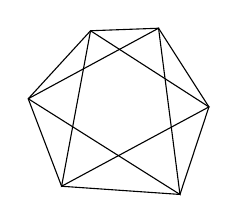
\begin{tikzpicture}[x=0.008cm,y=-0.008cm]
\draw (0,108)--(99,0)--(207,-4)--(287,121)--(241,260)--(53,247)--cycle;
\draw[thin] (0,108)--(207,-4)--(241,260)--(0,108);
\draw[thin] (99,0)--(53,247)--(287,121)--(99,0);
\end{tikzpicture}}

\[
\unsure{\nu|v}(\lambda)\nu(\lambda^{-1})\overset{?}{=}1
\]

\[
\begin{aligned}
\lambda^{-2}\nu(\lambda)&=\nu(\lambda^{-1})\overset{?}{=}\nu(\lambda)^{-1}\\
&\nu(\lambda)^2=\lambda^2\quad\overset{\text{donc}}{\Longrightarrow}\boxed{\nu(\lambda)\in(\mathbb Z/n\mathbb Z)^*}
\end{aligned}
\]

% archive sheet number: 290
\scanpage{292}

% letterhead
UNIVERSITE DES SCIENCES\\
ET TECHNIQUES DU LANGUEDOC\\
AMATHEMATIQUES

14.05.80

\uline{SEMINAIRE $\mathbb C^n$}

Monsieur C.-C. CHOU, Professeur à l'Université de Perpignan parlera sur

\uline{La notion de résidu}\qquad Lundi 19 mai 1980 à 10 h, Salle 331.

et sur

\uline{L'intégrale de Bochner-Martinelli}\qquad Lundi 2 juin 1980 à 10 h, Salle 331.

% archive sheet number: 291
\scanpage{293}

$\begin{pmatrix}\lambda&0\\0&\lambda^{-1}\end{pmatrix}$ normalisa\unsure{teur|tion} de $U_0$ opère sur $U_0$, par $\boxed{\lambda^2}$

et $\lambda:\mathrm{Et}(s)\xrightarrow{\sim}\mathrm{Et}(\lambda^{-1}s)$ qui transforme $\omega_s$ pour une orientation fixée en $\omega_{\lambda^{-1}s}^{\boxed{\lambda^2}}$ i.e.

\[
\boxed{\lambda\cdot(a\dotplus\zeta)=\lambda a+\lambda^2\zeta}
\]

Donc on ne récupère là que $\lambda^2$, pas $\lambda$ ! Mais la relation d'incidence entre $a\underset{s}{\dotplus}\zeta\in\mathrm{Et}(s)$ et $\lambda a\underset{\lambda^{-1}s}{\dotplus}\zeta'$ est

\[
\deleted{a}\quad\zeta'=\lambda^2\zeta\pm\lambda
\]

i.e. les quantités $\zeta'-\underset{\text{\uline{connu}}}{\underline{\lambda^2}}\zeta$ forment \unsure{l'ens|l'ens.|l'élém.} $\{\pm\lambda\}$ !

\noindent\rule{\linewidth}{.35pt}

\[
\zeta,\zeta'\ \text{incidents}\qquad\zeta'=\pm\lambda\qquad\deleted{\lambda\zeta}\qquad t'\pm\unsure{\nu|v}_{\lambda}
\]

\figure{\begin{tikzpicture}[x=.84cm,y=.84cm]
\draw (0,0)--(1.57,.37) (1.72,.07)--(3.25,.07) (3.42,.20)--(4.75,-.27);
\foreach \x/\y in {0/0,1.57/.37,3.18/.36}{\fill (\x,\y) circle (1.3pt);}
\node[below] at (0,0) {$s$};\node[above] at (1.57,.37) {$t$};\node[above right] at (3.18,.36) {$\lambda t=t'$};
\node at (1.75,.07) {$\deleted{a}$};\node at (3.15,.07) {$\deleted{\lambda a}$};
\node[right] at (4.75,-.27) {$\lambda^{-1}s=s'$};
\draw[very thin] (3.34,.22)..controls (1.09,-2.83) and (6.90,-4.41)..(8.16,-1.91)
..controls (9.40,.59) and (7.78,-.3)..(8.15,.12)
..controls (8.39,3.13) and (5.3,3.47)..(3.34,.22);
\node[right] at (8.62,1.0) {$\deleted{\unsure{a_0}}$};
\end{tikzpicture}}

\margin{$\mu(\lambda)$}

\figure{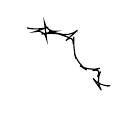
\begin{tikzpicture}[x=0.008cm,y=-0.008cm]
\draw[rounded corners] (0,0)--(15,4)--(27,0)--(28,8)--(38,6)--(50,9)--(65,15)--(73,8)--(71,31)--(78,57)--(97,69)--(119,62)--(106,84)--(113,94)--(125,92);
\end{tikzpicture}}

\[
\begin{aligned}
\zeta'_1&=\lambda^2\zeta+\lambda & \left\{\begin{aligned}\zeta'_1+\zeta'_2&=2\lambda^2\zeta\\\zeta'_1-\zeta'_2&=2\lambda\end{aligned}\right.\\[-1.8ex]
\zeta'_2&=\lambda^2\zeta-\lambda
\end{aligned}
\]

\[
\boxed{\underset{\substack{\rotatebox{90}{$\in$}\\\mathrm{Et}(s)}}{a}\ \text{incident :}\quad \lambda(a)\underset{\lambda^{-1}(s)}{\overset{\cdot}{\pm}}\underset{\substack{\rotatebox{90}{$\in$}\\\Lambda}}{\lambda}}
\]

\figure{\begin{tikzpicture}[x=0.008cm,y=-0.008cm]
\draw (0,0)--(162,-9);
\node[right] at (162,-9) {$s'$};
\end{tikzpicture}}

% archive sheet number: 292
\scanpage{294}

\diagram{\begin{tikzcd}[ampersand replacement=\&]
\mathrm{Et}(s)\arrow[rr,"\lambda"] \& \& \mathrm{Et}(\lambda^{-1}s)\\
\shortparallel \& y\longmapsto\lambda y \& \shortparallel\\
\{y\mid x\wedge y=e\} \& \& \{y'\mid\lambda^{-1}x\wedge y'=e\ \text{i.e.}\ x\wedge y'=\lambda e
\end{tikzcd}}

Relation entre $y,y'$

\[
y\wedge y'\unsure{\in|\subseteq}\pm e
\]

\[
\boxed{\lambda(y\dotplus\zeta)=\lambda y\dotplus\lambda^2\zeta}
\]

\margin{\uline{à prouver}}

et $\mathrm{Et}(s)$ torseur sous $\Lambda$ par

\[
y\dotplus\zeta=y+\zeta x
\]

$\mathrm{Et}(\lambda^{-1}s)$ torseur sous $\Lambda$ par

\[
y'\dotplus\zeta=y+\zeta(\lambda^{-1}x)=y+(\lambda^{-1}\zeta)x
\]

\[
\text{\uline{NB}}\qquad\lambda(y\dotplus\zeta)=\lambda(y+\zeta x)=\lambda y+\lambda\zeta x=\lambda y\dotplus(\lambda^2\zeta)
\]

Relation \deleted{$\unsure{y'_0=|y'_0|y_0}$} entre $\mathrm{Et}(s)$, $\mathrm{Et}(\lambda^{-1}s)$

\[
y\wedge y'\in\pm e
\]

\[
\begin{aligned}
y&=y_0\dotplus\zeta\ \unsure{=|=_{3}}\ y_0+\zeta x\\
y'&=y'_0\dotplus\zeta'=y'_0+(\lambda^{-1}\zeta')x
\end{aligned}
\]

\[
y'_0=\lambda y_0\quad\text{d'où }y'_0\wedge y_0=0
\]

\[
y\wedge y'=(\lambda\zeta-\lambda^{-1}\zeta')e
\]

\[
\begin{aligned}
\varphi(\zeta,\zeta')&=\lambda\zeta-\lambda^{-1}\zeta'\quad\in\pm1\\
&\left\{\begin{aligned}
\varphi(\zeta,\zeta')&=\varphi(\zeta+\alpha,\zeta'+\lambda^{\unsure{\alpha|2}}\alpha)\\
\varphi(\zeta,\zeta')&
\end{aligned}\right.
\end{aligned}
\]

\[
\boxed{\unsure{\xi'|\zeta'}=\lambda^2\xi\pm\lambda}\qquad\xi'
\]

% archive sheet number: 293
\scanpage{295}

\[
\begin{aligned}
&(y_0+\zetax)(y'_0+\zeta'\overset{\lambda^{-1}}{x})\\
&=(\lambda\zeta-\lambda^{-1}\zeta'+\unsure{\theta|\Theta})e
\end{aligned}
\]

\[
\deleted{\unsure{\lambda}}\zeta-\zeta'+\theta\in\pm1
\]

\[
\boxed{\lambda\zeta-\lambda^{-1}\zeta'+\theta\in\pm1}
\]

\[
\zeta'=\underbrace{\lambda^2\zeta+\underset{\substack{\text{\uline{dépend des}}\\\text{\uline{origines choisies}}}}{\underline{\lambda\theta}}}\pm\lambda
\qquad\zeta\in\mathbb Z/n\mathbb Z
\]

ops $\theta=0$

\[
\boxed{\mathrm{Et}(s)\xrightarrow{\overset{\lambda}{\sim}}\mathrm{Et}(\lambda^{-1}s)}
\qquad\lambda\zeta-\lambda^{-1}\zeta'
\]

\[
(s,\deleted{\lambda}t)\in A_0\Longleftrightarrow\{\lambda t,\lambda^{-1}s\}\in A_0
\]

\[
\begin{aligned}
\lambda\unsure{\xi|\zeta}-\lambda^{-1}\xi'&\in\pm1 &\alpha+\zeta&\qquad\lambda\alpha+\zeta'\\
&&\zeta-\lambda^{-1}\zeta'&
\end{aligned}
\]

\[
\begin{aligned}
\deleted{\lambda(\zeta+a)}&\qquad \unsure{t_0|t}\qquad\lambda t\\
\deleted{s}\qquad\lambda(t+\zeta)&=\deleted{\lambda(t+\zeta)}\,\lambda t+\lambda^2\zeta\\
\deleted{\unsure{a}}\quad t+\zeta&\qquad\lambda t+\zeta'\\
\lambda\unsure{\zeta|J}\unsure{-|\pm|\deleted{=}-}\lambda^{-1}\zeta'&\in\pm1
\end{aligned}
\]

\[
\lambda(\alpha+\zeta)-\lambda^{-1}(\lambda^2\alpha+\zeta')\in\pm1
\]

\[
\begin{aligned}
\deleted{\unsure{t+-}}\quad(t+\alpha)+\zeta&=&\lambda(t+\alpha)+\zeta'&\\
&=t+(\alpha+\zeta) & &=\lambda t+(\lambda^2\unsure{\alpha|2}+\zeta')
\end{aligned}
\]

% archive sheet number: 294
\scanpage{296}

\[
T_\lambda(A_{\lambda'})=A_{\lambda\lambda'}
\]

$\lambda$ \uline{\unsure{défini|définie|définit}} par $\unsure{\nu|v}$

$\lambda'$ \uline{défini} par $\nu'$

\[
\begin{aligned}
\mathrm{Et}_0(\lambda^{-1}t)&=\{s\in S\mid\{s,\lambda^{-1}t\}\in A_0\}\\
&=\{s\in S\mid\{s,t\}\in A_\lambda\}
\end{aligned}
\]

\[
\deleted{(}\{s,t\}\in A_{\unsure{\lambda|1}}\ \Longrightarrow\ \{\lambda
\]

$\nu(A_0,\lambda)$ défini par la condition

\[
\{s,t
\]

\[
E\unsure{,|.|{}}\in\unsure{\mathcal E|\mathscr E}\qquad A_{\unsure{i_E|iE|i,E|\in E}}
\]

\[
\deleted{\unsure{\mathbb Z|E}}
\]

% printed form
MR LE PROFESSEUR GROTHENDIECK ALEX.\\
MATHEMATIQUES\hfill 5

% archive sheet number: 295
\scanpage{297}

% letterhead
\begin{center}
U N I V E R S I T E\\
DES SCIENCES ET TECHNIQUES\\
DU LANGUEDOC\\
\texttt{------------}
\end{center}

MONTPELLIER, le 26 Juin 1980

Service de la Scolarité\\
MR/GJ\\
Diffusion : Liste H\\
N°: 3713

% printed form
\uline{AVIS DE SOUTENANCE D'UNE THESE DE DOCTORAT D'ETAT}

\uline{Nom et prénom du candidat} :TOUBOUL André

\uline{Titre de la thèse} : ``Caractérisation d'un dispositif à transfert de charges (S.C.C.D.) Transfert et bruit de fond par traitement numérique''.

\uline{Date, heure et lieu de soutenance prévus} : 11 JUILLET 1980 à 10 H. 30 mn\\
Salle de cours n° 9\\
(Bâtiment Administratif)

\uline{Nom des Directeurs de thèse} : Professeur G. LECOY et A.A. WALMA

\uline{Désignation du laboratoire où la thèse est préparée} : G.E.M.C.E.S.-C.E.E.S. (U.S.T.L.)

\uline{Résumé de la thèse} : Après avoir rappelé le fonctionnement d'un dispositif à transfert de charges (C.C.D.) à canal en surface, on présente une méthode numérique originale de mesure du bruit de fond menant directement à la variance des charges.Des mesures de bruit sont données : elles montrent la prépondérance des mécanismes de transfert sur le bruit. Pour certains modes de fonctionnement, le produit de l'inefficacité de transfert par la taille du paquet peut rendre compte de la variance des charges de bruit. L'influence des modes d'injection des charges ainsi que du taux de remplissage des puits a été mise en évidence. Pour expliquer le comportement du bruit et de l'inefficacité de transfert, on a suggéré que le rôle de la structure amorphe de l'interface soit considéré.

\uline{Durée approximative des recherches ayant abouti à la thèse} : 6 ans

\uline{Nom des rapporteurs} :

M. SAVELLI M., Professeur, E.E.A., U.S.T.L.

M. LECOY G., Professeur, E.E.A., U.S.T.L.

\unsure{M.|Mme} WALMA Alle Anne, Professeur Associé, E.E.A., U.S.T.L.

M. HOBSON G.S., Professeur, Electrical Eng., Université de Sheffield (G.B.)

\uline{Composition du jury proposé} :

M. SAVELLI, E.E.A., Professeur, U.S.T.L.  (Président)

M. BOREL, Directeur Recherche et Développement EFCIS, GRENOBLE

M. CAMUS , Directeur, CNET (Meylan-Grenoble)

M. DUMONTET, Phys. Sol. \& Phys. At, Professeur, U.S.T.L.\\
(Membre étranger à la spécialité du candidat)

M. HOBSON, Electrical Eng., Professeur, Univ. Sheffield (G.B.)\\
(Membre extérieur choisi en raison de sa compétence scientifique)

M. NOUGIER, E.E.A, Professeur, U.S.T.L.

M. LECOY, E.E.A., Professeur, U.S.T.L.

M. WALMA ,E.E.A., Professeur associé, U.S.T.L.

P. le Secrétaire Général,\\
L'Attachée d'Administration Universitaire,

\handwritten{\unsure{Gentil}}

\uline{A. GENTIL}

% archive sheet number: 296
